% !TEX TS-program = xelatex
% !TeX encoding = UTF-8

% \documentclass[master]{seuthesis} % 硕士

% 取消颜色,打印时候使用 !!!!!!!!!!!!
\documentclass[master,nocolorlinks]{seuthesis} 
% \documentclass[doctor]{seuthesis} % 博士
% \documentclass[engineering]{seuthesis} % 工程硕士

\usepackage{CJK,CJKnumb}
\usepackage{amsmath}
\usepackage{amsfonts}
\usepackage{amssymb}
\usepackage{bm}
\usepackage{subfigure}
\usepackage{url}
\usepackage{booktabs}
\usepackage{longtable}
\usepackage{multirow,makecell}
\usepackage{enumitem}
\usepackage{breqn}
\usepackage{mathrsfs}
\usepackage{tikz}
\usepackage{datetime}
\renewcommand{\today}{2021~年~5~月~25~日}
\renewcommand{\todayeng}{May , 2021}

\newtheorem{theorem}{定理}[chapter]
\newtheorem{lemma}{引理}[chapter]
\newtheorem{proof}{证明}[chapter]
\newtheorem{remark}{注}[chapter]
\newtheorem{definition}{定义}[chapter]

\graphicspath{{./image/}}
%\DeclareMathOperator{\sign}{sign} 

\begin{document}
\categorynumber{TP391} % 分类采用《中国图书资料分类法》
\UDC{621.3}            %《国际十进分类法UDC》的类号
\secretlevel{公开}      % 学位论文密级分为"公开"、"内部"、"秘密"和"机密"四种
\studentid{18xxxx}   %学号要完整,前面的零不能省略。

\title{基于深度学习的希腊字母研究}{{\color{red}学位论文形式:应用研究(专业硕士专用)}}{Thesis Title}{subtitle}
\author{朴智新}{Zhixin PIAO}
\advisor{杨绿溪}{教授}{Luxi YANG}{Prof.}
%\coadvisor{李春国}{教授}{LI Chunguo}{Prof.}  % Associate  Prof.  副教授

%\committeechair{徐琴珍 \quad 教授}
%\reader{黄永明 \quad 教授}{ 李春国 \quad 教授 }


\degree{工学硕士}
\major[12em]{信息与通信工程}  
\submajor{信号与信息处理}
\defenddate{\today}
\authorizedate{}
\department{信息科学与工程学院}{School of Information Science and Engineering}
%\duration{2017年1月—2017年6月}
%\address{中国无线谷5号楼2楼5212室}

%\thanks{本论文获国家XXX计划项目(2012AA00A00)和国家杰出青年科学基金项目(01234567)资助。}

\maketitle

% 中文、英文摘要
% !TeX root = ../main.tex
% !TEX TS-program = xelatex
% !TeX encoding = UTF-8


\begin{abstract}{希腊字母,腓尼基字母,语言,深度学习}
希腊字母源自腓尼基字母。腓尼基字母只有辅音,从右向左写。希腊语的元音发达,希腊人增添了元音字母。因为希腊人的书写工具是蜡板,有时前一行从右向左写完后顺势就从左向右写,变成所谓“耕地”式书写,后来逐渐演变成全部从左向右写。字母的方向也颠倒了。罗马人引进希腊字母,略微改变变为拉丁字母,在世界广为流行。希腊字母广泛应用到学术领域,如数学等。

希腊字母是希腊语所使用的字母,是世界上最早的有元音的字母,也广泛使用于数学、物理、生物、天文等学科。俄语等使用的西里尔字母也是由希腊字母演变而成。希腊字母进入了许多语言的词汇中,英语单字“alphabet”(字母表),源自拉丁语“alphabetum”,源自希腊语“αλφαβητον”,即为前两个希腊字母α(“Alpha”)及β(“Beta”)所合成,三角洲(“Delta”)这个词就来自希腊字母Δ,因为Δ是三角形。
\end{abstract}

\begin{englishabstract}{Greek Alphabet, Phoenician Alphabet, Language, Deep Learning}
The Greek alphabet has been used to write the Greek language since the late 9th century BC or early 8th century BC It was derived from the earlier Phoenician alphabet, and was the first alphabetic script to have distinct letters for vowels as well as consonants. It is the ancestor of the Latin and Cyrillic scripts.Apart from its use in writing the Greek language, in both its ancient and its modern forms, the Greek alphabet today also serves as a source of technical symbols and labels in many domains of mathematics, science and other fields.

In its classical and modern forms, the alphabet has 24 letters, ordered from alpha to omega. Like Latin and Cyrillic, Greek originally had only a single form of each letter; it developed the letter case distinction between upper-case and lower-case forms in parallel with Latin during the modern era.
\end{englishabstract}




\tableofcontents
% 专用术语的注释表
% !TeX root = ../main.tex
% !TEX TS-program = xelatex
% !TeX encoding = UTF-8


% 专用术语的注释表

\begin{terminology}
% \renewcommand\arraystretch{1.5}
\begin{longtable}{p{7cm}p{5cm}p{2cm}<{\centering}}  %{>{\normalsize}m{0.2\textwidth} <{\centering}m{0.7\textwidth}}
英文 & 中文 & 缩略词 \\
Artificial Intelligence & 人工智能     & AI \\
\end{longtable}
\end{terminology} 


\renewcommand{\listfigurename}{插图目录}
\renewcommand{\listtablename}{表格目录}
\listofothers

\begin{Main}
	% !TeX root = ../main.tex
% !TEX TS-program = xelatex
% !TeX encoding = UTF-8



\chapter{前言}
\section{数学公式}
\subsection{简单的数学公式}
\textbf{卷积}(\textbf{convolution})在图像分析的线性方法中是一种重要的运算。卷积是一个积分,反映一个函数$f(t)$在另一个函数上$h(t)$移动时所重叠的量。函数$f$和$h$在有限域$[0,t]$上的$1D$卷积$f*h$由下式给出:
 $$(f*h)(t) \equiv \int_0^t {f(\tau )h(t - \tau )d\tau } $$

\subsection{带自动编号的公式}
这里可以限定在$[0,t]$区间,原因是我们假设负坐标部分的值是0。为了准确起见,我们还可以将卷积积分的上限扩展为$( - \infty ,\infty )$:
\begin{equation}(f*h)(t) \equiv \int_{ - \infty }^\infty  {f(\tau )h(t - \tau )d\tau }  = \int_{ - \infty }^\infty  {f(t - \tau )h(\tau )d\tau }
  \end{equation} 

\subsection{带等号对齐的公式}
卷积可以推广到更高维。令$2D$函数$f$和$h$的卷积$g$记为$f*h$,则有:
\begin{equation}
\begin{aligned}
(f*h)(x,y) &= \int_{ - \infty }^\infty  {\int_{ - \infty }^\infty  {f(a,b)h(x - a,y - b)} } dadb\\
 &= \int_{ - \infty }^\infty  {\int_{ - \infty }^\infty  {f(x - a,y - b)h(a,b)} } dadb\\
\end{aligned}
\end{equation}

\section{伪代码}
在写论文的时候我们通常要写伪代码,伪代码里面有时甚至还要包含数学公式(如根号一类的)。伪代码会自动找一个比较好的位置插入图片。

\begin{algorithm}
    \caption{用归并排序求逆序数}
    \begin{algorithmic}[1] %每行显示行号
        \Require $Array$数组,$n$数组大小
        \Ensure 逆序数
        \Function {MergerSort}{$Array, left, right$}
            \State $result \gets 0$
            \If {$left < right$}
                \State $middle \gets (left + right) / 2$
                \State $result \gets result +$ \Call{MergerSort}{$Array, left, middle$}
                \State $result \gets result +$ \Call{MergerSort}{$Array, middle, right$}
                \State $result \gets result +$ \Call{Merger}{$Array,left,middle,right$}
            \EndIf
            \State \Return{$result$}
        \EndFunction
        \State
        \Function{Merger}{$Array, left, middle, right$}
            \State $i\gets left$
            \State $j\gets middle$
            \State $k\gets 0$
            \State $result \gets 0$
            \While{$i<middle$ \textbf{and} $j<right$}
                \If{$Array[i]<Array[j]$}
                    \State $B[k++]\gets Array[i++]$
                \Else
                    \State $B[k++] \gets Array[j++]$
                    \State $result \gets result + (middle - i)$
                \EndIf
            \EndWhile
            \While{$i<middle$}
                \State $B[k++] \gets Array[i++]$
            \EndWhile
            \While{$j<right$}
                \State $B[k++] \gets Array[j++]$
            \EndWhile
            \For{$i = 0 \to k-1$}
                \State $Array[left + i] \gets B[i]$
            \EndFor
            \State \Return{$result$}
        \EndFunction
    \end{algorithmic}
\end{algorithm}

\section{插入图片}
在使用该命令的时候,图片会自动找一个他觉得比较好的位置插入图片,我们就不需要担心前面改了文字之后后面的格式乱掉。
\begin{figure}[htbp!]
\centering 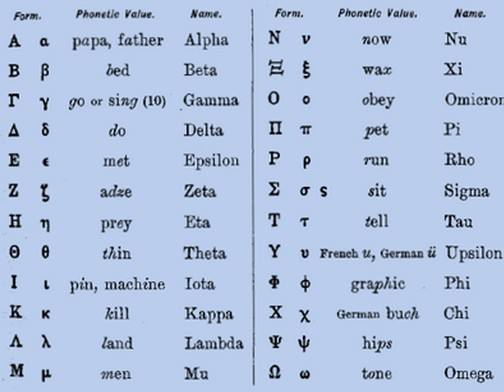
\includegraphics[width=0.9\textwidth]{image/test.jpg} \caption{图片的一个简单应用场景}
\end{figure}

\section{引用论文}
使得论文符合要求\cite{Yao:2015ix,seucover}。






	% !TeX root = ../main.tex
% !TEX TS-program = xelatex
% !TeX encoding = UTF-8


\chapter{背景综述}\label{chap-bg}



\section{cnn}



\section{目标检测}


	% !TeX root = ../main.tex
% !TEX TS-program = xelatex
% !TeX encoding = UTF-8



\chapter{自己的第一个点}
\section{数学公式}







	% !TeX root = ../main.tex
% !TEX TS-program = xelatex
% !TeX encoding = UTF-8



\chapter{自己的第二个点}
\section{数学公式}







	% !TeX root = ../main.tex
% !TEX TS-program = xelatex
% !TeX encoding = UTF-8



\chapter{自己的第三个点}
\section{数学公式}







	% !TeX root = ../main.tex
% !TEX TS-program = xelatex
% !TeX encoding = UTF-8



\chapter{未来与展望}
\section{数学公式}







\end{Main}

\begin{Acknowledgement}{}
% !TeX root = ../main.tex
% !TEX TS-program = xelatex
% !TeX encoding = UTF-8




% 感谢语

首先,我要感谢我的导师杨绿溪.

\end{Acknowledgement}

% 参考文献
\bibliographystyle{ref/thuthesis-numeric}
\bibliography{ref/seuthesis}


%\newpage
%\printindex % 索引

% 附录
\begin{Appendix}
% !TeX root = ../main.tex
% !TEX TS-program = xelatex
% !TeX encoding = UTF-8



\chapter{附录}
\section{数学公式}







\end{Appendix}

% 个人简介
\begin{Resume}
% !TeX root = ../main.tex
% !TEX TS-program = xelatex
% !TeX encoding = UTF-8



\begin{flushleft}
\textbf{\Large 学术论文}

[1] 论文

[2] 论文

\end{flushleft}
\hspace{2cm}

\begin{flushleft}
\textbf{\Large 申请专利}

[1] 专利

[2] 专利

\end{flushleft}

\end{Resume}
\end{document}





